\chapter[The \picomed Framework: A Modular Framework for Hypothesis-Driven Language Model Research]{The \picosupabig Framework: A Modular Framework for Hypothesis-Driven Language Model Research}
\label{chapter:pico}

% The rapid progress of large language models (LLMs) has produced systems that excel at a wide range of natural language tasks, from reasoning and summarization to coding and multilingual translation \citep{hendrycks2021mmlu, cobbe2021gsm8k, srivastava2023bigbench}. Yet this progress has also introduced new challenges: as models grow larger and more complex, they become harder to analyze, diagnose, and refine. Developing language models as a result is typically more of an art than a science.

This chapter introduces \pico, a framework designed to transform language model development from empirical guesswork into a rigorous scientific process. \pico enables researchers to systematically observe learning dynamics, formulate testable hypotheses about model behaviour, and iterate on design choices through controlled experimentation. By bridging the gap between training and analysis in a single, accessible framework, \pico makes it possible to build language models in a more principled, hypothesis-driven manner.\footnote{Code available at: \url{https://github.com/pico-lm}.} 

Existing model development frameworks such as DeepSpeed \citep{rasley2020deepspeed} and Megatron-LM \citep{narayanan2021megatron} have focused on efficient, large-scale training. However, their emphasis on production performance and throughput often comes at the cost of transparency. Intermediate representations, gradients, and activations are rarely captured in a structured way, and instrumentation for fine-grained interpretability is typically an afterthought. As a result, researchers seeking to study learning dynamics or test training interventions face steep technical overhead.

Conversely, frameworks built for interpretability, such as TransformerLens \citep{nanda2022transformerlens}, and model suites such as Pythia \citep{biderman2023pythia} enable detailed circuit-level analysis but are mostly limited to post-hoc exploration of fully trained models. They rarely support modifications to the training process itself, and when they do, such interventions tend to be tightly coupled to specific checkpoints, architectures, or datasets. Even frameworks explicitly designed for developmental analysis, like DevInterp \citep{devinterpcode}, rely on external checkpointing pipelines and are often decoupled from model training.

To support scientific research on language models, researchers need infrastructure that both logs advanced training signals (activations and gradients) and also invites easy experimentation and modification of the training process. Crucially, this framework should be lightweight and accessible and prioritise iteration speed over engineering overhead. 

\paragraph{Chapter Contributions} \pico is a modular, extensible framework designed to fill the gap between training and analysis for small language models. Built for training and analysing small-to-medium scale models (1M--1B parameters), \pico is engineered to support the scientific methodology demonstrated in the previous chapter: systematic observation, hypothesis generation, controlled experimentation, and iterative refinement. It consists of two components:

\begin{enumerate}
    \item \texttt{pico-train}, a customisable training library that simplifies training models from scratch while recording rich internal signals (weights, gradients, activations) at regular checkpoints.
    \item \texttt{pico-analyze}, a companion toolkit for querying, visualising, and analysing these signals—designed to integrate smoothly with standard scientific workflows and support user-defined metrics.
\end{enumerate}

Together, these tools make it possible to perform fine-grained, in-situ analysis of how models learn over time, test hypotheses about representation development, and prototype interventions that might improve training outcomes. This is particularly important for small models, where interpretability and efficiency are especially critical.

% \pico was built to address a concrete gap identified in the previous chapter: existing suites like Pythia offer rich insights into learning dynamics after training, but lack the flexibility and transparency needed to test interventions during training. The findings from \cref{chapter:tending-towards-stability} (e.g. the correlation between effective rank and convergence speed) generate specific, testable hypotheses that require tools for systematic experimentation. \pico provides these tools, bringing the same level of rigor to the training process as to post-hoc analysis.

\paragraph{Addressing RQ2} This chapter addresses the second research question of this thesis, by developing a novel framework framework that supports scientific research on language models. This framework makes the process of training and analysing language models more scientific and accessible to a wider range of researchers.

\vspace{1em}

The rest of this chapter is structured as follows. \cref{sec:pico-related} situates \pico within the broader ecosystem of language model training and interpretability frameworks, reviewing both large-scale production platforms and experimental research toolkits. \cref{sec:pico-overview} describes the key architectural and design decisions behind \texttt{pico-train} and \texttt{pico-analyze}, highlighting how they support training-time experimentation. \cref{sec:pico-demo} runs through a basic toy demonstratino of \pico; finally \cref{sec:pico-case-studies} demonstrates \pico's value through two case studies that show how it enables researchers to systematically test and refine hypotheses about language model learning dynamics.

{
\renewcommand{\arraystretch}{1.25}
\setlength{\tabcolsep}{4pt}

\begin{table}[htbp]
    \centering
    \footnotesize
    \begin{tabular}{@{}p{2.7cm} p{1.7cm} p{2.4cm} p{2.3cm} p{2.3cm} p{2.2cm}@{}}
    \toprule
    \textbf{Tool} &
    \textbf{Custom \newline Training} &
    \textbf{Checkpoint \newline Support} &
    \textbf{Feature \newline Extraction} &
    \textbf{Analysis \newline Tools} &
    \textbf{Low-Budget \newline Friendly} \\
    \midrule
    \textbf{\pico} & 
    \cmark \newline Modular \newline PyTorch &
    \cmark \newline Optimizer, \newline weights \& data &
    \cmark \newline Activations \& \newline gradients &
    \cmark \newline \texttt{pico-analyze} \newline metrics &
    \cmark \newline Academic \newline GPU-scale \\

    \midrule

    TransformerLens & 
    \xmark & \xmark & \cmark & \cmark & \cmark \\

    ACDC & 
    \xmark & \xmark & \cmark & \cmark & \cmark \\

    SAELens & 
    \xmark & \xmark & \warnmark & \cmark & \cmark \\

    \midrule

    SmolLM2 & 
    \cmark & \warnmark & \xmark & \xmark & \cmark \\

    Pythia Suite & 
    \warnmark & \warnmark & \xmark & \warnmark & \cmark \\

    OLMo & 
    \cmark & \warnmark & \xmark & \xmark & \warnmark \\

    \bottomrule
    \end{tabular}

    \caption{Comparison of \pico and related frameworks for interpretability and learning dynamics. 
    \label{tab:pico_comparison} \newline
    \textbf{Legend:} \cmark = Fully supported; \warnmark = Partial; \xmark = Not supported.}
\end{table}
}

\section[Situating \picomed Among Language Model Frameworks]{Situating \picolarge Among Language Model Frameworks}
\label{sec:pico-related}

Language model research increasingly depends on infrastructure that supports both scaling up training and opening up models to analysis. As interest grows in how models acquire structure, allocate capacity, and evolve over time, researchers need frameworks that support more than just efficient training. They need transparency into the training process itself.

To understand the niche \pico fills, I situate it relative to two major categories of tools: training frameworks and analysis frameworks.
% Today's ecosystem of LLM tooling is rich but uneven. On one end are large-scale training platforms that emphasize throughput, hardware optimisation, and production readiness, these include DeepSpeed \citep{rasley2020deepspeed}, Megatron-LM \citep{narayanan2021megatron}, and MosaicML's MPT \citep{mosaic2023mpt}. On the other are interpretability toolkits that provide detailed post-hoc analysis of model internals, often at the level of neurons, circuits, or activations, such as TransformerLens \citep{nanda2022transformerlens}, ROME \citep{meng2022locating}, and ACDC \citep{conmy2023towards}. However, few systems support both perspectives simultaneously. \pico is designed to bridge this gap. It supports full training from scratch, while offering built-in mechanisms to log and analyze activations, gradients, and other internal signals throughout training. This makes it possible to study learning dynamics not only retrospectively, but as they unfold which can then inform future design choices.


\paragraph{Training Frameworks}
Large-scale systems like Megatron-LM \citep{narayanan2021megatron}, DeepSpeed \citep{rasley2020deepspeed}, and MosaicML \citep{mosaic2023mpt} are highly optimised for training massive models. They handle distributed computation and mixed-precision arithmetic efficiently, but their training pipelines are complex and often opaque. Modifying or instrumenting them to inspect model internals (let alone run repeated training interventions) can require significant effort. These frameworks are indispensable for production-scale pretraining, but ill-suited for small-scale, experiment-driven research.

In contrast, lightweight training frameworks such as NanoGPT \citep{karpathy2023nanogpt}, SmolLM2 \citep{allal2025smollm2}, TinyLlama \citep{zhang2024tinyllama}, and TinyStories \citep{eldan2023tinystories} emphasise simplicity and fast iteration. Their codebases are accessible and easy to modify, making them ideal for prototyping new ideas. However, they tend to treat training as a black box. Logging activations or inspecting weight evolution generally requires manual modification, and internal state tracking is minimal or absent. These frameworks make it easy to run experiments, but hard to measure what is happening inside.

%\pico aims to combine the best of both worlds. It is optimised for small and mid-sized models (1M--1B parameters) and is built in modular PyTorch for ease of use. But unlike most lightweight suites, it is designed from the ground up to expose model internals. It logs key training signals by default (weights, activations, gradients) and does so in structured, extensible formats. %This makes \pico not just a tool for training models, but a platform for studying how they learn.

\paragraph{Analysis Frameworks}
Where training frameworks help build models, analysis frameworks help interpret them. Recent progress in mechanistic interpretability has produced tools like TransformerLens \citep{nanda2022transformerlens}, ROME \citep{meng2022locating}, and ACDC \citep{conmy2023towards}, which allow detailed inspection of trained transformer circuits. These tools are useful for understanding among other things how attention heads specialise or how knowledge is stored and retrieved. But they are mostly post-hoc: they assume a trained model and operate over static checkpoints.

Model suites such as Pythia \citep{biderman2023pythia} and OLMo \citep{groeneveld2024olmo} provided researchers a set of pretrained models and training checkpoints to study. Rather than having to train a model from scratch, researchers can use these models to analyse the learning dynamics of a model that has already been trained, using consistent checkpoints and data. However, these frameworks are not designed to retrain models from scratch.

Complementing the frameworks above are tools like DevInterp \citep{devinterpcode}, which begin to trace how models develop during training by analysing intermediate checkpoints. This shift toward developmental interpretability has revealed that models undergo discrete representational shifts and acquire capabilities in phases \citep{hoogland2023towards, hoogland2025losslandscape}. However, all of these frameworks remain downstream of the training process; they depend on external training pipelines and cannot modify or influence the training process itself.

% Here again, \pico closes a key loop. By integrating training and analysis into the same workflow, it enables fine-grained, in-situ investigation of representational dynamics. Rather than relying on occasional checkpoints saved by another framework, \pico makes detailed logging a native part of the training loop. This allows researchers to monitor changes in capacity usage, representation similarity, or sparsity metrics in real time, and to test hypotheses by intervening directly in training.

\paragraph{Toward Integrated Research Infrastructure}
The distinctions between training and analysis frameworks have historically reflected different goals—efficiency vs. interpretability, scale vs. visibility. But to understand how language models learn, especially at small and intermediate scales, these goals need to be brought together. \pico is an attempt to unify them into a single research workflow, one that enables controlled experimentation, rapid iteration, and structured analysis without sacrificing clarity or flexibility.

\cref{tab:pico_comparison} provides a comparative summary of how \pico fits into the current landscape, alongside other commonly used frameworks. While each tool has strengths of its own, \pico is distinct in offering custom training, rich logging, and built-in analysis all in one package.

\section[\picomed]{\picolarge}
\label{sec:pico-overview}

In this section I provide a concise overview of the two \pico libraries: \texttt{pico-train} and \texttt{pico-analyze}. 

\subsection{\texttt{pico-train}: A Minimalist Approach to Model Training}

\texttt{pico-train} is a lightweight, transparent framework for training small- to medium-scale language models. Unlike many existing training libraries that prioritise efficiency at the cost of clarity, \texttt{pico-train} is designed to be simple, modular, and easy to modify. This makes it a flexible foundation for experimentation in language model research.

Out of the box, \texttt{pico-train} implements \texttt{pico-decoder}, a LLaMA-style transformer \citep{touvron2023llama} that incorporates key features of modern auto-regressive language models, including Grouped Query Attention (GQA) \citep{ainslie2023gqa}, Rotary Position Embeddings (RoPE) \citep{su2024rope}, FlashAttention \citep{dao2022flashattention}, SwiGLU activations \citep{shazeer2020glu}, and RMSNorm \citep{zhang2019rmsnorm}. All components (except FlashAttention) are re-implemented from scratch in plain PyTorch \citep{paszke2017pytorch}, with an emphasis on readability and documentation. %Future iterations of \pico will introduce additional architectures, such as \texttt{pico-diffusion} and \texttt{pico-statespace} models, all adhering to the same guiding principle: every \texttt{pico-*} model must be simple, well-documented, and serve as a clear base implementation for the given model architecture.

To ensure efficient multi-GPU and distributed training, \texttt{pico-train} is built on Lightning Fabric \citep{lightning-fabric}. Lightning Fabric enables users to scale up training across multiple GPUs or nodes without introducing excessive abstractions and ensures that the core training logic remains easy to understand and modify.

A distinguishing feature of \texttt{pico-train} is its systematic checkpointing and version control system. It automatically saves:
\begin{itemize}
    \item \textbf{Model states in both PyTorch- and Hugging Face-compatible formats} \citep{huggingface}. This dual-format checkpointing enables straightforward loading with vanilla PyTorch or integration into the Hugging Face ecosystem, facilitating downstream tasks such as fine-tuning, inference, or model sharing. Researchers can thus easily plug \texttt{pico-train} outputs into existing pipelines or community projects.

    \item \textbf{Intermediate activations and gradients.} At user-defined intervals, the library gathers layerwise activations and gradients from the forward and backward passes on the current training batch. Optionally, it can also capture these metrics from a fixed evaluation batch for consistent comparisons over training. Collecting these tensors at each checkpoint provides a granular record of how representations and gradient flows evolve over time.

    \item \textbf{Evaluation results.} During training, \texttt{pico-train} records user-defined evaluation metrics (e.g., validation perplexity or accuracy) alongside model checkpoints.
\end{itemize}
\vspace{-0.2em}
All checkpoints are automatically uploaded and version-controlled on Hugging Face, ensuring that researchers can revisit any point in training to analyse how the model evolved over time. These structured checkpoints integrate seamlessly with \texttt{pico-analyze}, enabling learning dynamics research with minimal setup.

\subsection{Pretokenized Dataset: \texttt{pretokenized-dolma}}

To simplify experimentation, I also release \textbf{\texttt{pretokenized-dolma}}: a pre-tokenized, pre-chunked, and pre-shuffled version of Dolma \citep{soldaini2024dolma}, a large, open-source English dataset. This dataset removes preprocessing overhead, ensures consistency across runs, and supports streaming to reduce storage needs. Using it is optional; users can substitute their own data if they prefer. 

To prepare the \textbf{\texttt{pretokenized-dolma}} dataset, I begin by downloading the Dolma corpus and selecting a random 30\% subset. The text is then tokenised using the open-sourced \textbf{\texttt{allenai/OLMo-7B-0724-hf}} tokenizer and split into fixed-length sequences of 2049 tokens (2048 + 1 for next-token prediction). I ensure consistency across shards by chunking token streams without overlap, dropping any remainder shorter than the full sequence length.

After tokenisation and chunking, I shuffle the dataset and sample a fixed number of sequences per shard, generating 100 shards in total. To facilitate scalable loading and training, I further fine-shard the dataset into 10,000 pieces using a secondary script. These final shards are compact (78MB each), randomly shuffled, pre-tokenized, and ready for streaming via the Hugging Face datasets API. This preprocessing ensures that all models see data in a consistent order, which is critical for learning dynamics analysis. I release all of the scripts used for preprocessing data in a GitHub repository. The resulting dataset is saved as Parquet files and uploaded to a Hugging Face organisation\footnote{\url{https://huggingface.co/pico-lm}} under \href{https://huggingface.co/datasets/pico-lm/pretokenized-dolma}{\textcolor{blue}{\textbf{\texttt{pico-lm/pretokenized-dolma}}}}.

The design philosophy for the dataset is the same as for \texttt{pico-train}: minimalism, modularity, and transparency, that enable users to easily modify all aspects of the training pipeline. 

\subsection{\texttt{pico-analyze}: A General-Purpose Framework for Studying Learning Dynamics}

\texttt{pico-analyze} is a companion tool to \texttt{pico-train} designed to make analysing learning dynamics seamless and reproducible. It directly integrates with the checkpoints saved by \texttt{pico-train}, including model weights, optimizer states, activations, and gradients, allowing researchers to systematically compute the learning dynamics of trained models.

At its core, \texttt{pico-analyze} follows a simple abstraction: it applies metrics to components. Metrics provide quantitative insights into various aspects of model behaviour, while components define the specific model elements being analysed. This design allows for flexible and fine-grained analysis of training dynamics. 

\paragraph{Metrics.} Out of the box, \texttt{pico-analyze} supports a range of built-in metrics. These include:
\begin{itemize}
    \item \textbf{Sparsity Measures}: \textit{Gini coefficient} \citep{hurley2009gini} and \textit{Hoyer metric} \citep{hoyer2004sparsity} gauge how concentrated the values of a tensor are around zero.

    \item \textbf{Rank-Based Metrics}: \textit{Proportional Effective Rank} (defined in Chapter 6) captures a matrix's “effective dimensionality”, while \textit{Condition Number} evaluates its numerical stability.

    \item \textbf{Representation Similarity}: \textit{CKA} \citep{kornblith2019cka} and \textit{PWCCA} \citep{morcos2018pwcca} compare activation patterns across layers or checkpoints, revealing how internal representations evolve.
    
    \item \textbf{Norms}: \textit{Frobenius}, \textit{Nuclear}, and \textit{Infinity} norms measure the scale of a tensor, spotlighting issues such as vanishing or exploding parameters.
\end{itemize}

\paragraph{Components.} Metrics can be computed on different types of components, which fall into two categories: 
\begin{itemize} 
\item \textbf{Simple components}: Individual weight matrices, gradients, or activations from a single layer. 
\item \textbf{Compound components}: Higher-level structures that combine multiple model elements. One example is the OV circuit, which tracks how information flows in transformer models by combining the value projection and output projection matrices in self-attention layers \cite{elhage2021mathematical}. 
\end{itemize}

This two-step abstraction is designed for extensibility: new metrics and component types can be easily defined, allowing researchers to tailor analyses to specific hypotheses about language model learning. Note that I provide a detailed explanation of all of the metrics in \cref{chapter:analysis-background}.

\section{Usage Demonstration} 
\label{sec:pico-demo}

To illustrate how \pico enables rigorous, hypothesis-driven research in practice, this section walks through a minimal end-to-end workflow. Rather than simply showing how to run code, this demonstration highlights how researchers can configure, train, and analyse small models to test specific learning dynamics hypotheses. \pico forms a closed scientific loop of observation, intervention, and refinement.

\subsection{Training Models with \texttt{pico-train}}

Setting up the \texttt{pico-train} codebase requires running the following commands:

\begin{center}
    \begin{codelisting}
        git clone https://github.com/pico-lm/pico-train.git
        cd pico-train
        echo "HF_TOKEN=your_huggingface_token" >> .env
        echo "WANDB_API=your_wandb_key" >> .env
        source setup.sh
    \end{codelisting}
\end{center}

I provide a simple \verb|setup.sh| script that uses Poetry \citep{poetry} to install dependencies and configure the environment. Training a model requires only a configuration file. \texttt{pico-train} uses flexible dataclasses with sensible defaults that can be easily customised for each run. I report all of the defaults in \cref{tab:default_configs}. For demonstration purposes, I include a sample configuration file in \texttt{pico-train} that can be found under \href{https://github.com/pico-lm/pico-train/blob/main/configs/demo.yaml}{\textcolor{blue}{\texttt{configs/demo.yaml}}}\footnote{\url{https://github.com/pico-lm/pico-train/blob/main/configs/demo.yaml}}. The toy model trained by this configuration is a tiny 11M parameter model, trained for only 100 steps. Here I show an abridged version of this configuration:


\begin{center}
    \begin{configlisting}
        data: # dataset and dataloading configurations
        checkpointing:
            run_name: "pico-decoder-demo-run"
            save_to_hf: true
            hf_checkpoint_id:
                repo_id: "pico-lm/demo"
        model: # model and model loading configurations
        evaluation: # evaluation configurations
        monitoring: # monitoring configurations
            save_to_wandb: true
            wandb:
                project: "pico-demo"
                entity: "pico-lm"
        training: # training configurations
    \end{configlisting}
\end{center}
% \begin{figure}[h!] 
%     \centering
%     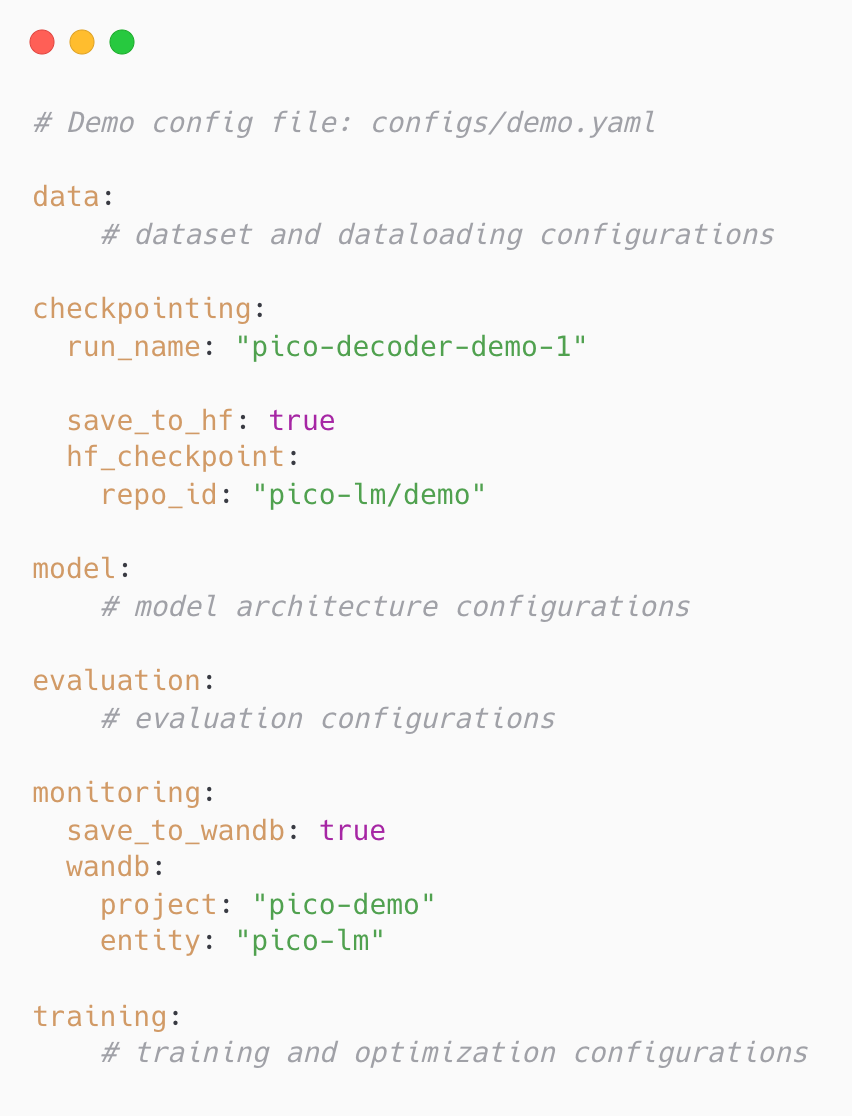
\includegraphics[width=0.7\columnwidth]{chapters/pico/figures/demo/demo_config.png}
%     \caption{The abridged demo configuration setup that we include with \texttt{pico-train}.}
%     \label{fig:demo_config}
% \end{figure}

In general, the configuration file consists of six main components, each controlling key aspects of model training. 

Using this demo configuration file, users can launch a training run as follows:

\begin{center}
    \begin{codelisting}
        poetry run pico-train --config_path configs/demo.yaml
    \end{codelisting}
\end{center}

Training will start immediately, automatically saving learning dynamics checkpoints both locally and on Hugging Face. In \cref{tab:default_configs}, I report the default configuration settings used in \texttt{pico-train}; users should refer to this table when configuring their own runs.

\begin{table*}[h!]
    \centering
    \renewcommand{\arraystretch}{1.2} % Adjust row spacing
    \setlength{\tabcolsep}{8pt} % Adjust column spacing
    \footnotesize
    \begin{tabular}{|>{\centering\arraybackslash}p{3cm}|p{5cm}|p{5.5cm}|}
        \hline
        \textbf{Category} & \textbf{Parameter} & \textbf{Default Value} \\
        \hline
        \multirow{10}{*}{\textbf{Model}}  
            & Model Type & \texttt{pico\_decoder} \\
            & Hidden Dimension ($d_{\text{model}}$) & 768 \\
            & Number of Layers ($n_{\text{layers}}$) & 12 \\
            & Vocabulary Size & 50,304 \\
            & Sequence Length & 2,048 \\
            & Attention Heads & 12 \\
            & Key/Value Heads & 4 \\
            & Activation Hidden Dim & 3,072 \\
            & Normalisation Epsilon & $1 \times 10^{-6}$ \\
            & Positional Emb. Theta & 10,000.0 \\
        \hline
        \multirow{7}{*}{\textbf{Training}}  
            & Optimizer & AdamW \\
            & Learning Rate & $3 \times 10^{-4}$ \\
            & LR Scheduler & Linear w/ Warmup \\
            & Warmup Steps & 2,500 \\
            & Gradient Accum. Steps & 128 \\
            & Max Training Steps & 200,000 \\
            & Precision & BF16 Mixed \\
            %& Accelerator & CUDA \\
            %& Nodes & 1 \\
            %& Devices per Node & 1 \\
        \hline
        \multirow{3}{*}{\textbf{Data}}  
            & Dataset Name & \texttt{pretokenized-dolma} \\
            & Batch Size & 1,024 \\
            & Tokenizer & \texttt{allenai/OLMo-7B-0724-hf} \\
        \hline
        \multirow{6}{*}{\textbf{Checkpointing}}  
            & Auto Resume & True \\
            & Save Every N Steps & 1,000 \\
            %& Save to Hugging Face & False \\
            & Learning Dynamics Layers & \texttt{"attention.v\_proj",} \newline \texttt{"attention.o\_proj",} \newline \texttt{"swiglu.w\_2"} \\
            & Learning Dynamics Data & \texttt{pretokenized-paloma-tinsy} \\
        \hline
        \multirow{3}{*}{\textbf{Evaluation}}  
            & Metrics & \texttt{["paloma"]} \\
            & Eval Dataset Name & \texttt{pretokenized-paloma-tinsy} \\
            & Eval Batch Size & 16 \\
        \hline
        \multirow{3}{*}{\textbf{Monitoring}}  
            & Logging Level & INFO \\
            & Log Every N Steps & 100 \\
            %& Save to Weights \& Biases & False \\
        \hline
    \end{tabular}
    \caption{Default configuration settings used in \texttt{pico-train}, organised by configuration category.}
    \label{tab:default_configs}
\end{table*}

\subsection{Analysing Models with \texttt{pico-analyze}}


Once training is complete, users can inspect various aspects of the model's learning dynamics using \texttt{pico-analyze}. The setup process mirrors that of \texttt{pico-train}, making it simple to switch between training and analysis within the same workflow. \texttt{pico-analyze} works directly on the structured checkpoints saved by \texttt{pico-train}, computing metrics on model weights, gradients, and activations to provide insights into how the model evolves during training. To streamline experimentation, it uses a YAML-based configuration system that lets users specify which layers, metrics, and training steps to analyse. I include a complete sample configuration at \href{https://github.com/pico-lm/pico-analyze/blob/main/configs/demo.yaml}{\textcolor{blue}{\texttt{configs/demo.yaml}}}\footnote{\url{https://github.com/pico-lm/pico-analyze/blob/main/configs/demo.yaml}} within the \texttt{pico-analyze} repository.

To illustrate how this works in practice, one part of the demonstration configuration uses Centered Kernel Alignment (CKA) to test how much the model's internal representations change over training. As discussed in \cref{chapter:analysis-background}, Centered Kernel Alignment (CKA) is a well-established metric for comparing the similarity of activations between layers, checkpoints, or even different models. In this demonstration, I use CKA to track the convergence of the OV circuit at the first and last layers of the model. In general, I would expect the CKA score to begin at a value close to 0 and increase over time as the representations converge to their final state. However, since this toy example only trains for 100 steps, I hypothesise that there should be little representational change, and the CKA score should remain relatively high. This illustrates how users of \pico can turn a vague question such as “are the representations of my model changing?” into a quantitative hypothesis.

Below is an abridged YAML configuration that specifies this CKA analysis:

\begin{center}
\begin{configlisting}
    metrics:
    - metric_name: cka # Centered Kernel Alignment
      target_checkpoint: 100
      data_split: "val"
      components: 
        - component_name: ov_circuit
          data_type: "activations"
          layer_suffixes: 
            output_layer: "attention.o_proj"
            value_layer: "attention.v_proj"
          layers: [0,11]

\end{configlisting}
\end{center}

As expected, when I inspect the automatically generated plots (see \cref{fig:demo_full_run}), I see that the CKA similarity changes very little between the start and end of training (top left plot); at the start of training, the representations in both layers are already over 96\% similar to their final representations. This confirms that the toy model has barely begun to learn meaningful representations and highlights the obvious next step: train the model for longer. While this insight is trivial in a toy example, the same process generalises to larger models and more complex training regimes. In the subsequent section, I illustrate this through two more advanced case studies. The takeaway is that this hypothesis-driven loop (define a question, run the experiment, iterate on model design) can be scaled up to iteratively develop better language models.

\begin{figure}[t]
    \centering
    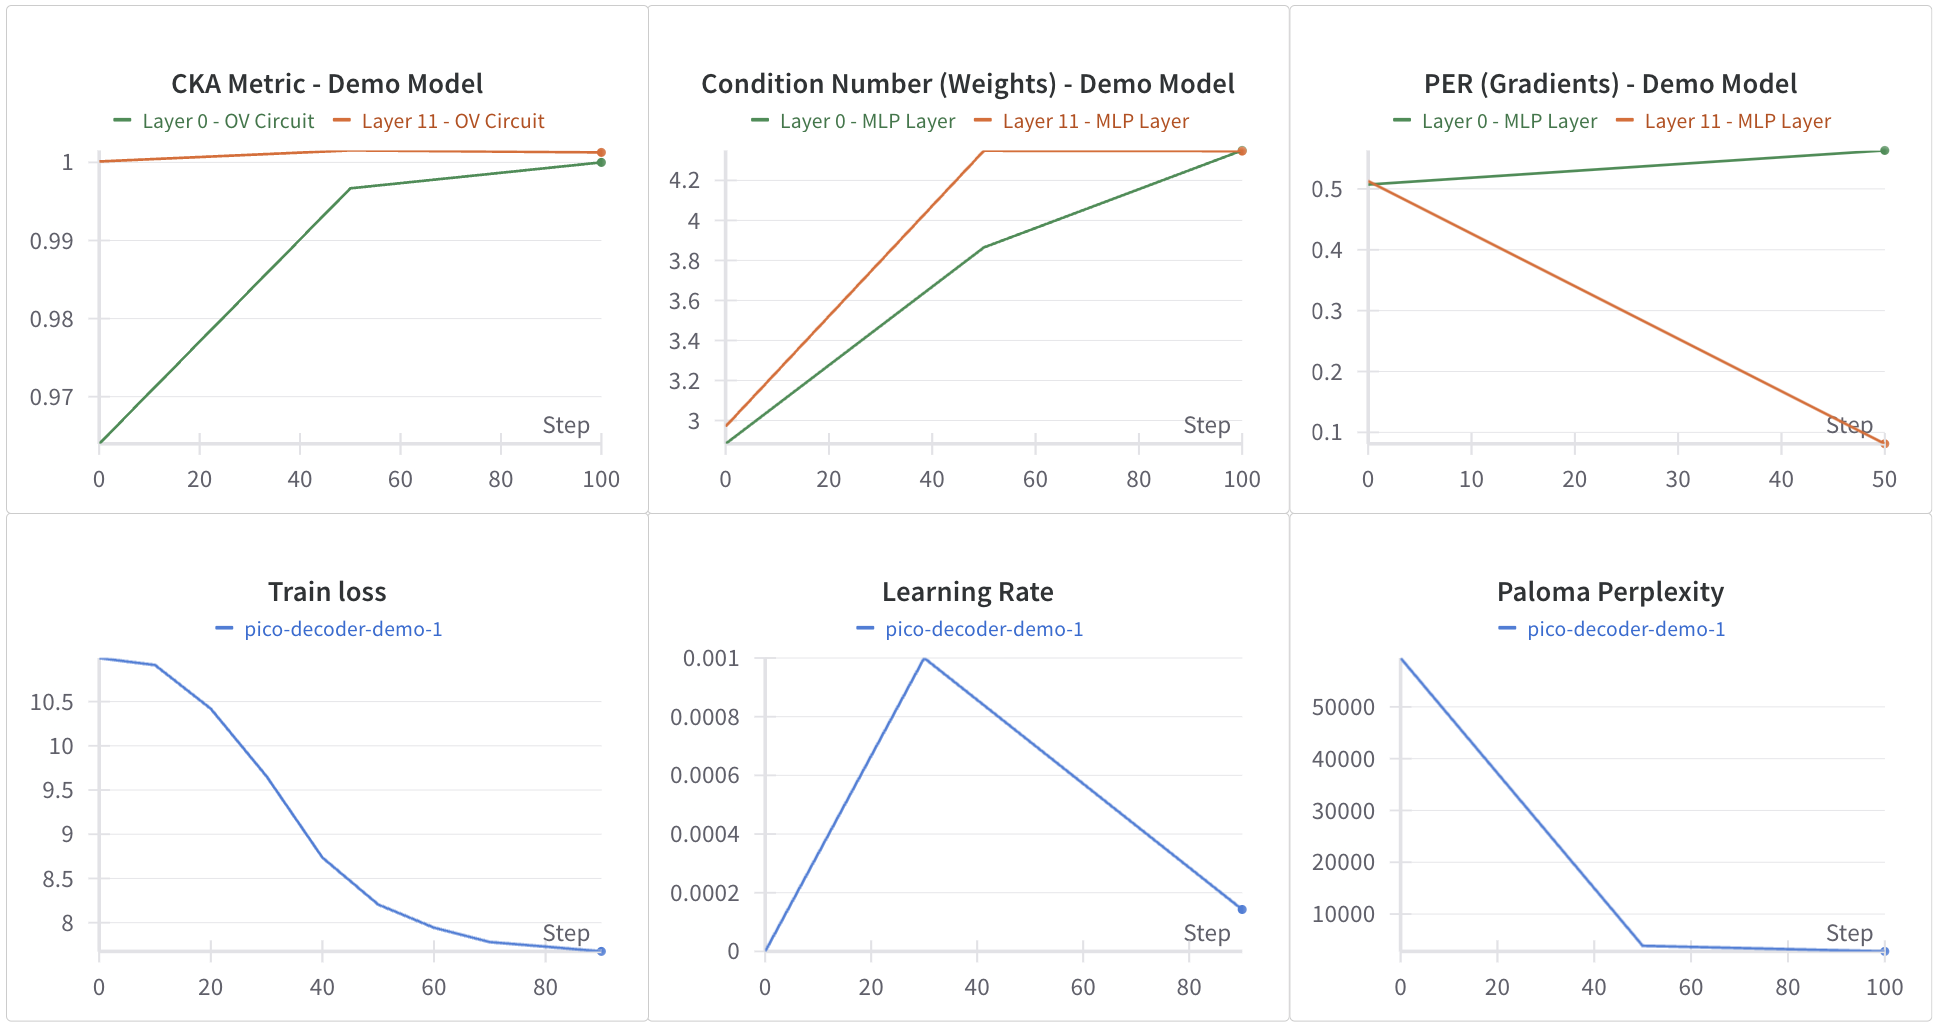
\includegraphics[width=0.9\textwidth]{chapters/pico/figures/demo_full_run.png}
    \caption{Sample analysis output of a dummy model trained using \texttt{pico-train} and analysed with \texttt{pico-analyze}. The top row illustrates some sample metrics computed by \texttt{pico-analyze} on the dummy model that was trained for 100 steps using \texttt{pico-train}, the bottom row shows training logs.}
    \label{fig:demo_full_run}
\end{figure}

In general, users can easily adapt these configuration files to test different metrics, components, or hypotheses. The full list of built-in metrics is provided in \cref{tab:pico_analyze_metrics}.

With a configuration file in place, launching an analysis is done as follows:

\begin{center}
    \begin{codelisting}
    poetry run pico-analyze
        --config_path configs/demo.yaml
        --repo_id pico-lm/demo
        --branch pico-decoder-demo-1
    \end{codelisting}
\end{center}

This command runs the specified analysis directly on the checkpoints uploaded by \texttt{pico-train}, using the given \verb|repo_id| and \verb|branch| to locate the training run. Results can be stored locally or automatically logged to Weights \& Biases (wandb) \citep{wandb} for comparison and visualisation.

By integrating seamlessly with \texttt{pico-train}, \texttt{pico-analyze} provides a structured, reproducible workflow for studying learning dynamics which inform model design choices.

\begin{table*}[h!]
    \centering
    \renewcommand{\arraystretch}{1.2} % Adjust row spacing
    \setlength{\tabcolsep}{4pt}
    \footnotesize
    \begin{tabular}{|p{4cm}|p{7.2cm}|p{1.9cm}|p{1.7cm}|}
        \hline
        \textbf{Metric} & \textbf{Description} & \textbf{Data Type} & \textbf{Category} \\
        \hline
        \hline
        \textbf{CKA \newline (Centered Kernel \newline Alignment)} \citep{kornblith2019cka} &  
        Measures similarity between activations at different checkpoints using kernel methods to track representation evolution. & Activations & \textbf{Similarity} \\
        \hline
        \textbf{PWCCA \newline (Projection-Weighted \newline CCA)} \cite{morcos2018pwcca} & 
        Measures activation similarity across training, emphasising important components via projections. & Activations & \textbf{Similarity} \\
        \hline
        \hline
        \textbf{Condition Number} &  
        Computes the ratio of largest to smallest singular value, indicating sensitivity to small input changes. & Weights\newline Activations\newline Gradients & \textbf{Rank} \\
        \hline
        \textbf{PER \newline (Proportional Effective Rank)} (Chapter 6) &  
        Measures entropy of normalised singular values to estimate effective parameter usage. & Weights\newline Gradients & \textbf{Rank} \\
        \hline
        \hline
        \textbf{Gini \newline Coefficient} \citep{hurley2009gini} &  
        Measures sparsity via inequality in the distribution of weights, activations, or gradients. & Weights\newline Activations\newline Gradients & \textbf{Sparsity} \\
        \hline
        \textbf{Hoyer's \newline Sparsity} \citep{hoyer2004sparsity} &  
        Measures sparsity using the ratio of L1 to L2 norms. & Weights\newline Activations\newline Gradients & \textbf{Sparsity} \\
        \hline
        \hline
        \textbf{Norm} &  
        Uses Frobenius, Nuclear, or Infinity matrix norms to quantify magnitude. & Weights\newline Activations\newline Gradients & \textbf{Norm} \\
        \hline
    \end{tabular}
    \caption{Overview of built-in metrics in \texttt{pico-analyze}. \textbf{Data Types} indicates on what types of checkpoint data the metrics can be applied. The \textbf{Category} column classifies metrics based on their primary purpose.}
    \label{tab:pico_analyze_metrics}
\end{table*}

\section{Case Studies}
\label{sec:pico-case-studies}

I illustrate how \pico enables systematic, hypothesis-driven experimentation through two case studies: (1) meta-learning pre-training, (2) low-rank adapter pre-training. In each of these examples, I demonstrate demonstrate the cycle of implementation, analysis, and hypothesis refinement.

\subsection{Meta-Learning Pre-Training}
\label{subsec:pico-meta-learning}

Model-Agnostic Meta-Learning (\citealp[MAML]{finn2017maml}) trains models to adapt quickly by alternating between short bursts of task-specific learning and a global update that improves generalisation. This setup encourages models to find initialisation points that adapt well to new tasks. While MAML is typically used for fine-tuning, I follow prior work \citep{bansal2020smlmt, li2021semisupervised} in applying it during pretraining.%, using synthetic token classification tasks.


\paragraph{Implementation} I implemented MAML in \texttt{pico-train} by adding a lightweight inner loop that updates a classification head on masked token tasks, followed by a meta-update to the full model. \texttt{pico-train} automatically handles distributed GPU synchronisation, requiring no changes to \pico's core training logic.

\begin{figure}[h!]
    \centering
    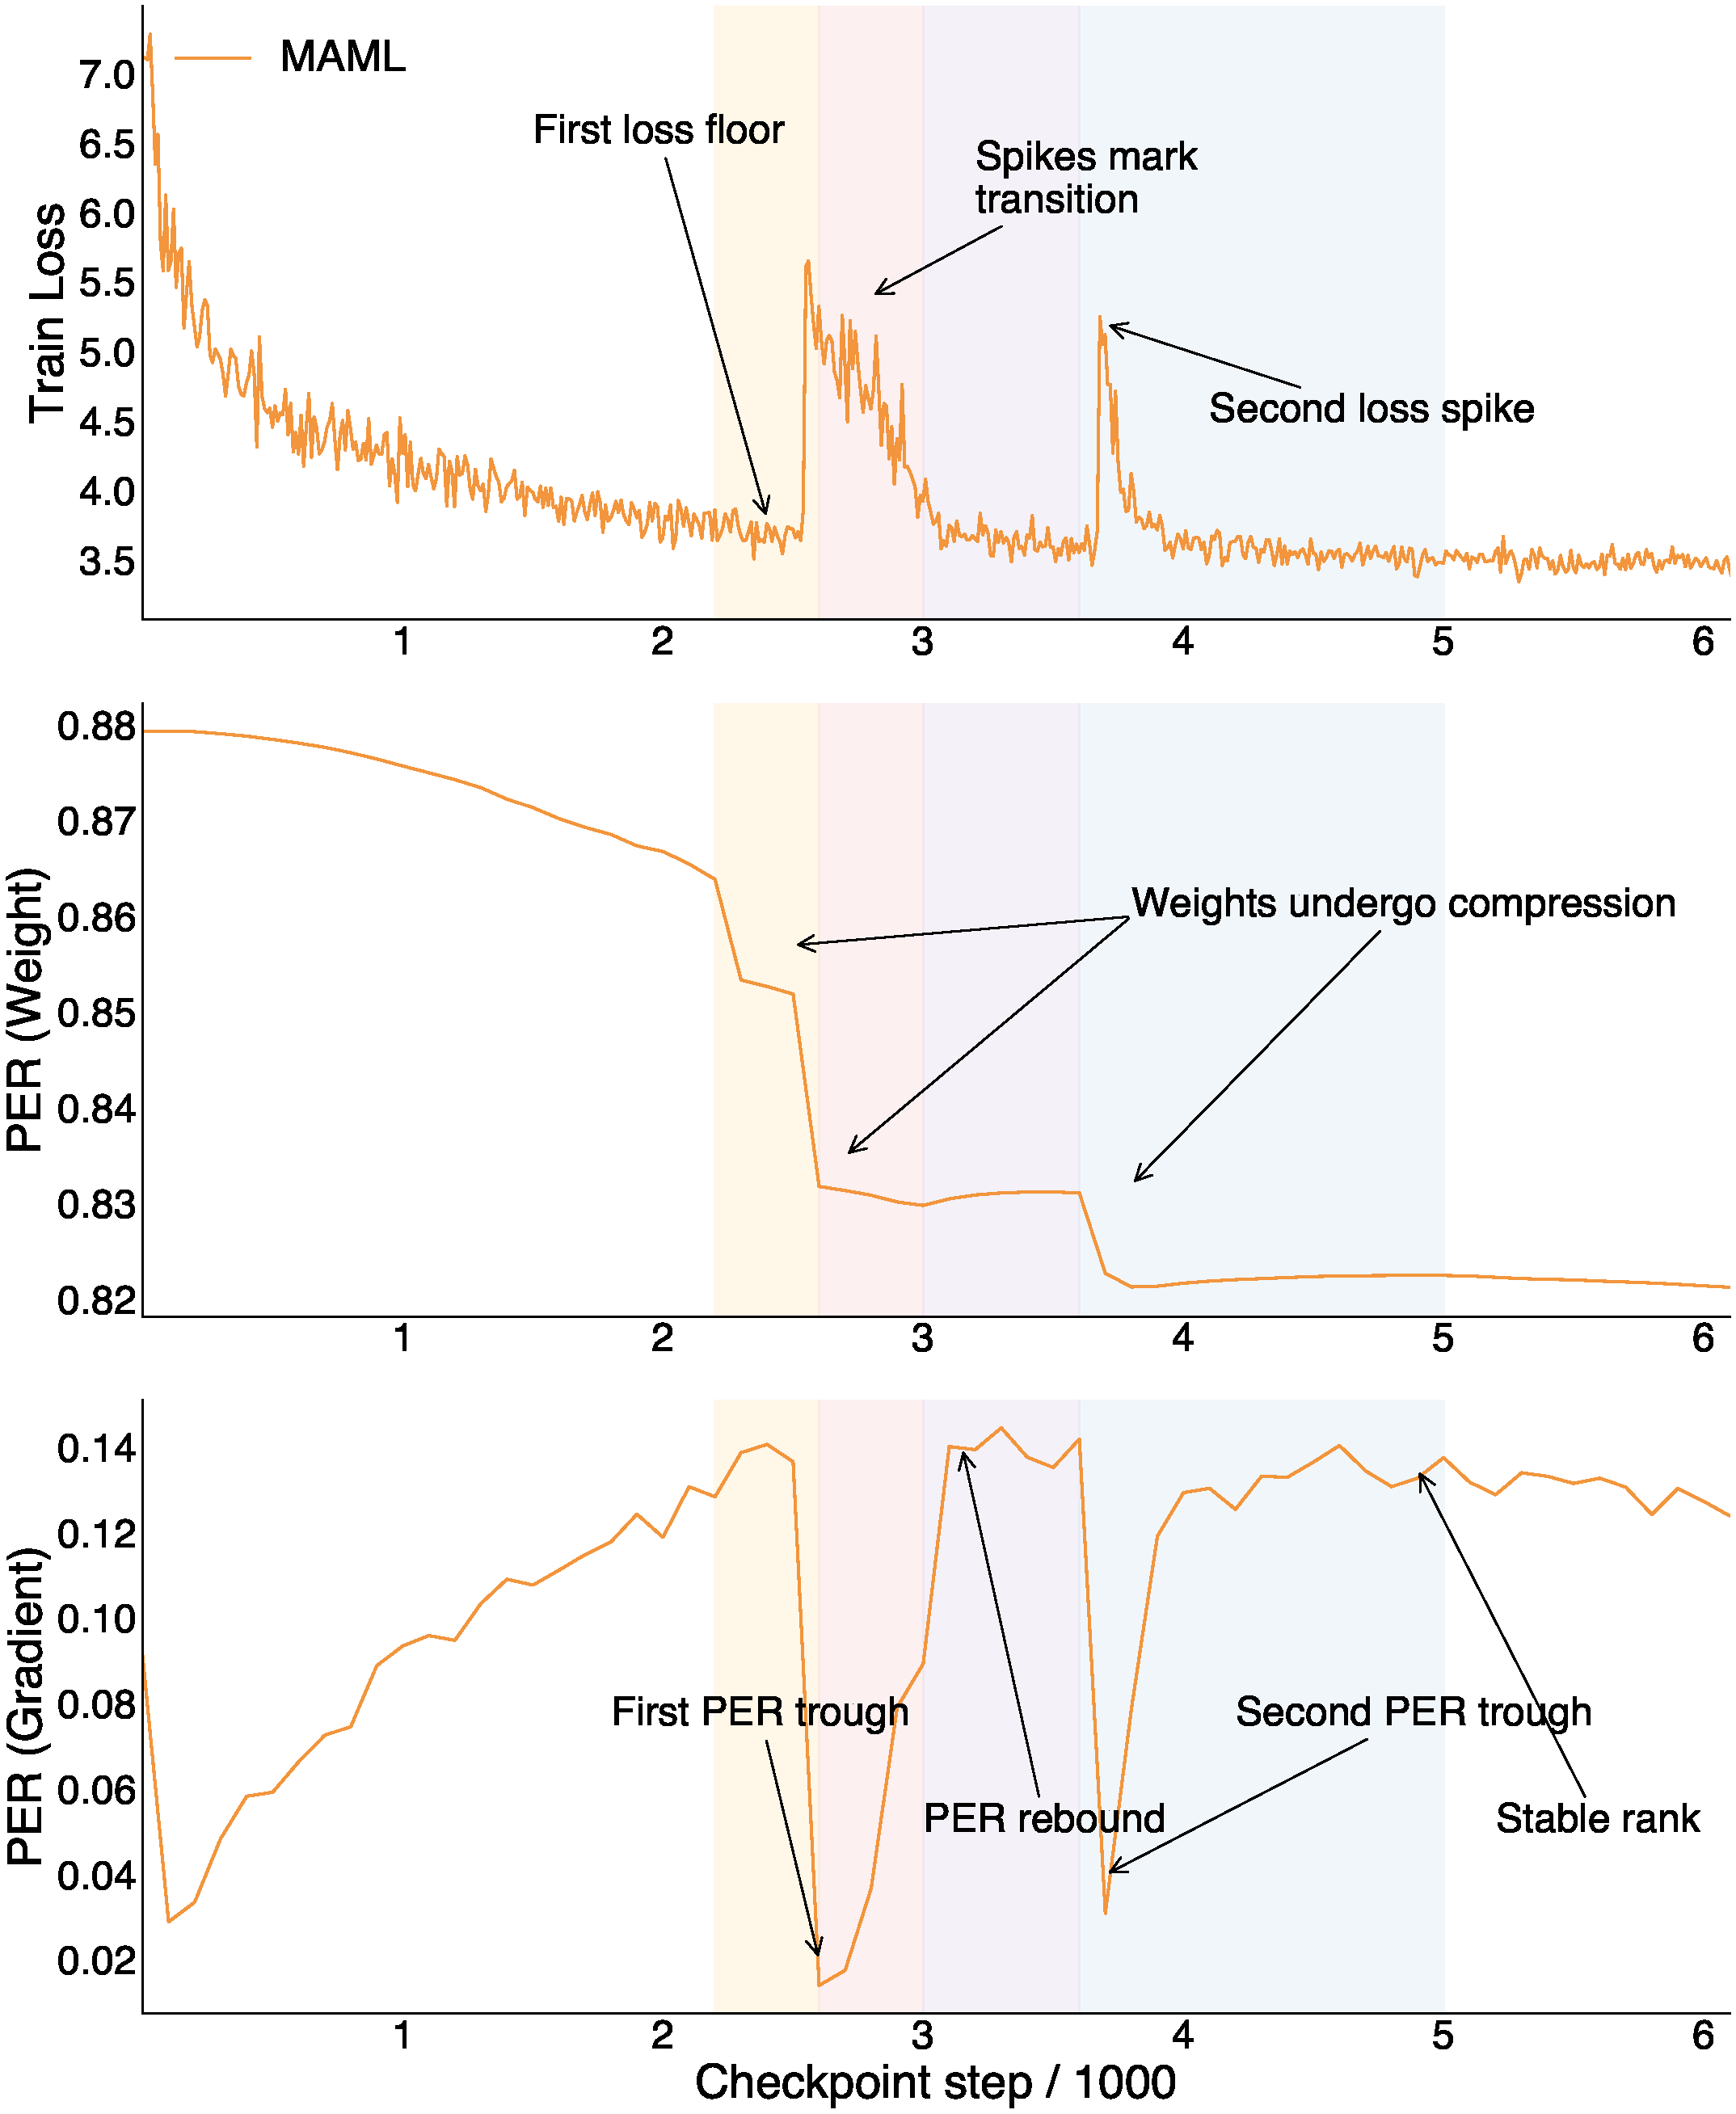
\includegraphics[width=0.6\textwidth]{chapters/pico/figures/maml-example.pdf}
    \caption{Training dynamics under MAML.
    \textbf{Top to bottom:} Training loss and proportional effective rank (PER) of weights and gradients.
    Sharp drops in PER align with spikes in loss. Shaded regions correspond to different observed phases in training. 
    }
    \label{fig:maml_example}
\end{figure}


\paragraph{Analysis} I evaluate MAML on Paloma perplexity and observe consistent 4-15\% gains over standard pretraining. To better understand this improvement, I analyse the proportional effective rank (PER) (defined in Chapter 6) of both weights and gradients over time. PER captures the dimensionality of a tensor's signal. In meta-learning, one concern is that inner-loop updates may overly constrain model updates to a low-dimensional subspace, potentially limiting generalisation. As shown in \cref{fig:maml_example}, I observe synchronised troughs in PER and spikes in both loss and perplexity. This suggests that inner-loop updates temporarily compress the model's capacity into a low-rank subspace before the outer-loop update restores variance and expressivity.


\paragraph{New Hypothesis and Next Steps}
These results support the hypothesis that MAML's learning dynamics involve cycles of compression and recovery. This raises concrete follow-up questions: could adjusting the inner-loop learning rate reduce excessive compression? Would alternative meta-learning schedules or task mixes stabilise the representational space more effectively? Using \pico's modular training and built-in logging, these variants can be tested with minimal friction. By comparing learning dynamics and outcomes across runs, researchers can refine their design choices in a reproducible, hypothesis-driven loop.% — illustrating Pico’s role as a practical sandbox for systematic small LM research.

\subsection{Low-Rank Adapter Pre-Training}
\label{subsec:pico-low-rank-adapter}

ReLoRA \citep{lialin2023relora} adapts LoRA \citep{hu2021lora}, a fine-tuning technique that freezes pretrained weights and injects trainable low-rank matrices, into the pretraining loop. In theory, this could provide a sample-efficient way to train large models by constraining updates to a low-rank subspace. %However, its impact on pretraining stability remains poorly understood.

\paragraph{Implementation} I incorporate ReLoRA into \texttt{pico-train} by adding a lightweight wrapper around attention and MLP weight matrices, and by modifying the learning rate schedule to handle periodic resets. I evaluated the model on BLiMP \citep{warstadt2020blimp}, which I configured via a single config entry. % and required minimal code modification. 

\begin{figure}[h!]
    \centering
    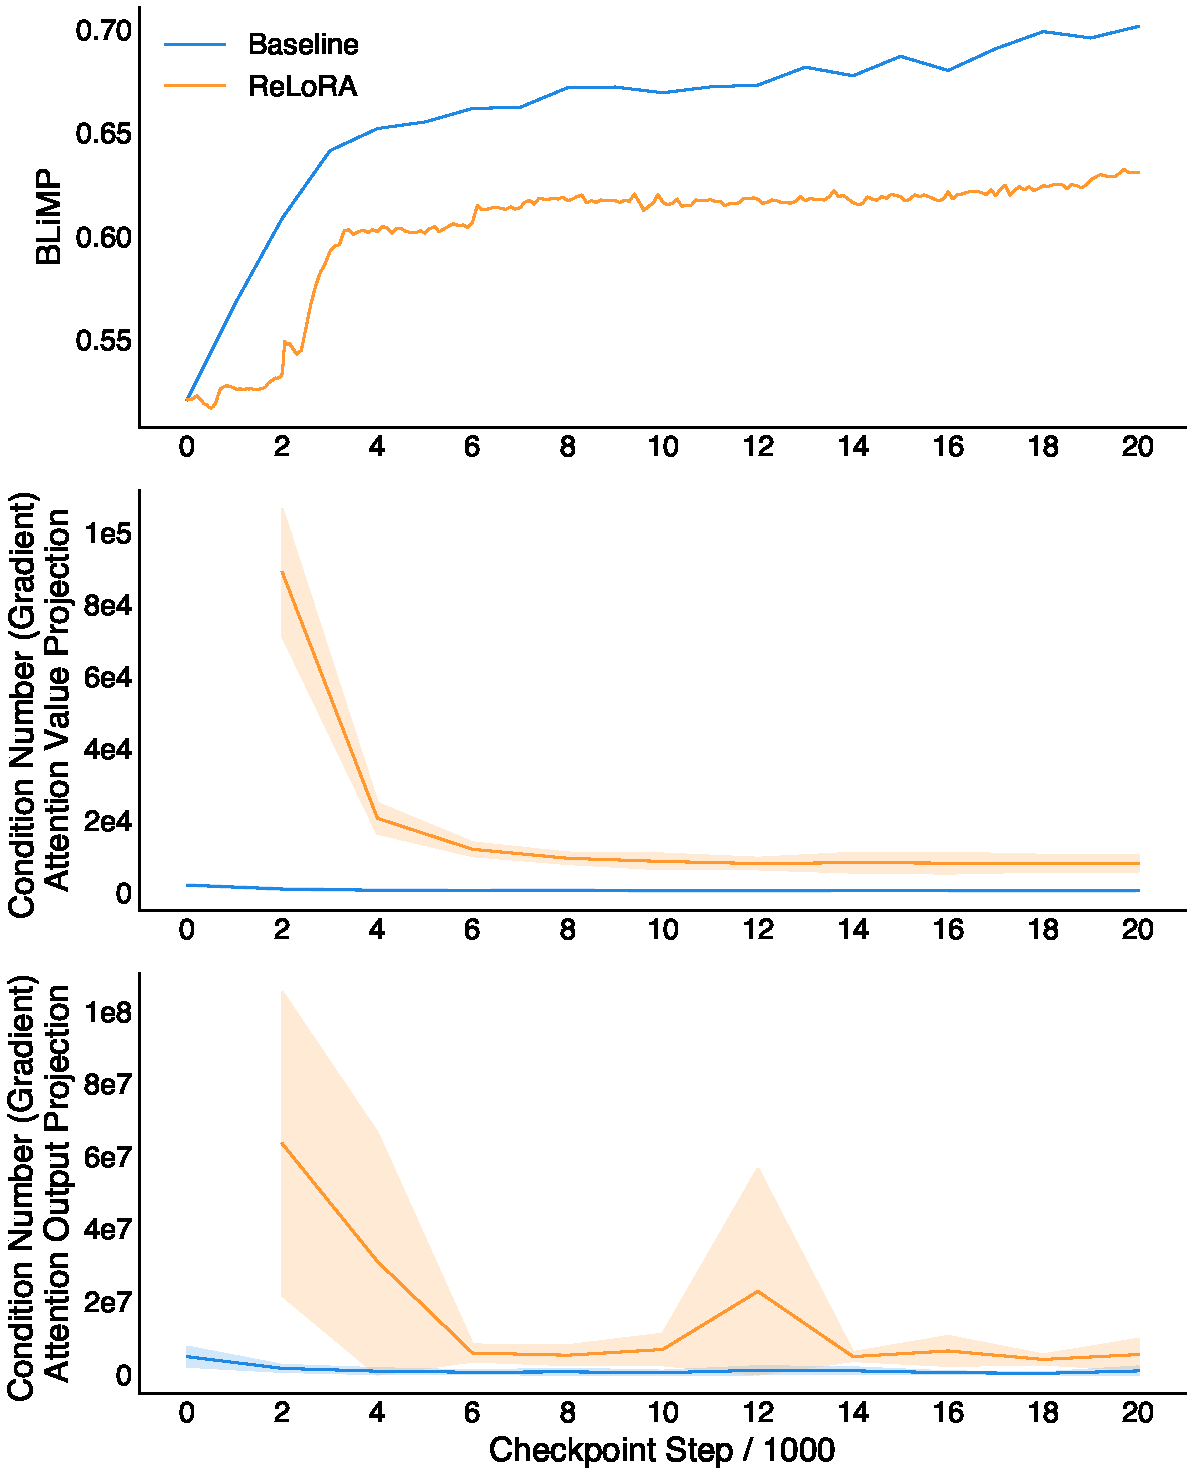
\includegraphics[width=0.6\textwidth]{chapters/pico/figures/relora-example.pdf}
    \caption{Training dynamics under ReLoRA.
    \textbf{Top to bottom:} BLiMP accuracy over time, averaged condition numbers of the gradient updates for the attention value and output projection matrices. Condition number shows wide inter-layer variance.
    }
    \label{fig:relora_example}
\end{figure}

\paragraph{Analysis} I find that ReLoRA surprisingly underperforms standard pretraining on BLiMP (see \cref{fig:relora_example}, top) \citep{warstadt2020blimp}. To investigate this, I analyse the condition numbers of the gradient updates across layers and training checkpoints. This metric reflects how sensitive gradient-based updates are to numerical instability, a relevant concern for methods like ReLoRA that repeatedly project updates into a low-rank subspace. As shown in \cref{fig:relora_example} (bottom), ReLoRA gradients are substantially more ill-conditioned and exhibit high inter-layer variance. 

% If the optimization geometry becomes poorly conditioned, learning can become more erratic.

\paragraph{New Hypothesis and Next Steps}
This pattern suggests that repeated low-rank resets may amplify gradient instability, undermining ReLoRA's intended efficiency gains. Several next steps follow naturally: for example, adding layerwise condition number regularisation, adjusting the rank dynamically, or modifying the reset schedule to reduce instability. Because \texttt{pico-train} and \texttt{pico-analyze} modularise core components and log detailed in-situ signals, researchers can test these changes quickly, track their effects on gradient stability, and iterate systematically. This demonstrates \pico's value as a scientific sandbox for implementing, analysing, and refining design choices in the small LM regime.

\section{Pico Model Suite}
\label{sec:pico-model-suite}

In addition to releasing the \texttt{pico-train} and \texttt{pico-analyze} tools, I also train a suite of \textbf{\texttt{pico-decoder}} models at various scales using \texttt{pico-train}, all of which are open-sourced on the Hugging Face organisation.\footnote{\url{https://huggingface.co/pico-lm}} These models range from 11M to 570M parameters, with plans to extend up to 1B, and serve both as evaluations of the training pipeline and as testbeds for research on scaling laws and interpretability. I provide a comparison of these models in \cref{tab:pico-decoder-configs}.

\begin{table}[h!]
    \centering
    \renewcommand{\arraystretch}{1.2}
    \begin{tabular}{|p{0.30\textwidth}||p{0.13\textwidth}|p{0.13\textwidth}|p{0.13\textwidth}|p{0.13\textwidth}|}
    \hline
    \multicolumn{5}{|c|}{\textbf{Pico-Decoder Model Comparison}} \\
    \hline
    \textbf{Attribute} & \texttt{tiny} & \texttt{small} & \texttt{medium} & \texttt{large} \\
    \hline
    Parameter Count & 11M & 65M & 181M & 570M \\
    Hidden Dimension ($d_{\text{model}}$) & 96 & 384 & 768 & 1536 \\
    Feed-forward Dim & 384 & 1536 & 3072 & 6144 \\
    Training Time (50K steps) & 10d 9h & 15d 6h & 17d 15h & 23d 16h \\
    \hline
    \end{tabular}
    \vspace{0.5em}
    \caption{Comparison of \texttt{pico-decoder} model variants trained with default \texttt{pico-train} configurations. Except for hidden and feed-forward dimension, all models share the training settings detailed in \cref{tab:default_configs}. Models are trained for 125,000 total training steps on 16 NVIDIA A100-SXM4-80GB GPUs.}
    \label{tab:pico-decoder-configs}
    \end{table}

Each model is trained for 125,000 steps (covering 250B tokens) on the open-sourced \textbf{\texttt{pretokenized-dolma}} dataset. I evaluate the final model checkpoints on the Paloma benchmark \citep{magnusson2024paloma}, HellaSwag \citep{zellers2019hellaswag}, Arc-Easy \citep{clark2018arc} and Truthful QA \citep{lin2022truthfulqa}, comparing performance against established decoder models. As shown in \cref{tab:model_benchmarks}, the models achieve comparable results to Pythia and OPT models, despite running on an academic-level compute budget (4 nodes of 4 A100s each). This illustrates that although simple and minimal, \texttt{pico-train} is able to efficiently train models that are competitive with state-of-the-art models of the same scale.

\begin{table*}[htbp!]
    \centering
    \renewcommand{\arraystretch}{1.1}
    \setlength{\tabcolsep}{6pt}
    \small
    \begin{tabular}{lcccccc}
    \hline
    \textbf{Family} & \textbf{Size} & \textbf{\#Tokens} &
    \textbf{Paloma$\;\downarrow$} &
    \textbf{HellaSwag$\;\uparrow$} &
    \textbf{ARC-Easy$\;\uparrow$} &
    \textbf{TruthfulQA$\;\uparrow$} \\
    \hline\hline
    
    \textbf{\pico} & 11M  & 250B & 136.17 & 25.62 & 32.79 & 51.75 \\
                   & 65M  & 250B &  42.24 & 27.25 & 38.22 & 46.13 \\
                   & 181M & 250B &  30.08 & 30.69 & 44.65 & 41.85 \\
                   & 570M & 250B &  22.96 & 37.33 & 48.99 & 36.33 \\
    \hline
    
    \textbf{Pythia} & 14M  & 300B &  86.64 & 26.15 & 31.31 & 50.14 \\
                    & 70M  & 300B &  43.76 & 27.56 & 36.23 & 47.02 \\
                    & 160M & 300B &  29.96 & 30.26 & 43.73 & 44.51 \\
                    & 410M & 300B &  20.55 & 40.55 & 52.10 & 41.23 \\
    \hline
    
    \textbf{OPT}    & 125M & 300B &  27.22 & 31.33 & 43.48 & 42.89 \\
                    & 350M & 300B &  20.91 & 36.66 & 44.06 & 41.01 \\
    \hline
    \end{tabular}
    \caption{Performance of small-scale language models on four benchmarks.
    Lower is better for Paloma perplexity ($\downarrow$); higher is better for
    HellaSwag, ARC-Easy, and Truthful QA accuracies ($\uparrow$).}
    \label{tab:model_benchmarks}
    %\vspace{-0.5cm}
\end{table*}

\section{Conclusion}
\label{sec:pico-conclusion}

% We introduce \pico, a modular framework for training and analyzing small to medium-scale language models. \texttt{pico-train} provides a minimal yet flexible environment for training language models that emphasises transparency and checkpointing for learning dynamics research. \texttt{pico-analyze} then uses these checkpoints to facilitate a broad set of learning dynamics analyses including model convergence patterns, sparsity, and rank dynamics.

% In addition, we presented the \pico Model Suite, a collection of  \textbf{\texttt{pico-decoder}} models ranging from 11M to 570M parameters, with future plans to scale to 1B+. These models are trained under controlled conditions, supporting research on scaling laws and representation learning.

% By bridging training and analysis in a lightweight, extensible framework, \pico lowers the barrier for studying language model learning dynamics. Future work will expand the model suite and integrate advanced interpretability tools, further enhancing its utility for rigorous and reproducible research.

In this chapter, I introduced \pico, a modular framework designed to transform language model development from empirical guesswork into a more rigorous, hypothesis-driven scientific process. By integrating transparent, checkpoint-rich training (\texttt{pico-train}) with systematic, reproducible analysis (\texttt{pico-analyze}), \pico bridges the gap between building models and understanding how they learn. In doing so, this chapter directly advances \textbf{RQ2}: \pico operationalises and makes accessible a novel scientific workflow for small LMs.

Unlike traditional frameworks that treat training and interpretability as separate, \pico combines them in a single, lightweight toolkit. This enables researchers to observe learning dynamics as they unfold, formulate concrete hypotheses about model behaviour, and test interventions in situ. The case studies and demonstration workflow show how this integrated loop makes language model research more principled and accessible.

The \pico Model Suite further supports this goal by providing open, reproducible checkpoints that serve as testbeds for scaling laws and interpretability research. By lowering the technical barriers to developmental analysis, \pico empowers researchers to study representation formation, capacity allocation, and training stability without requiring industrial-scale compute.

Looking ahead, my goal is to expand \pico with additional architectures and more analysis tooling to make language model research more systematic, transparent, and reproducible.


\vspace{1em}
For convenience, I provide links to the \pico Model Suite, the \pico GitHub repository, the \pico website, and the \pico demo video.

\begin{center}
    \begin{tblr}{
      colspec = {X[c] X[c] X[c] X[c]},
      colsep = 4pt,
      stretch = 0
    }
      \parbox{3.6cm}{
        \centering
        \raisebox{-0.4em}{
\includegraphics[width=1.9em]{chapters/pico/figures/assets/huggingface-logo.png}}\\
        {\footnotesize\href{https://huggingface.co/pico-lm}{\textcolor{blue}{huggingface.co/pico-lm}}}\\
        {\tiny (Apache 2.0)}
      }
      &
      \parbox{3.2cm}{
        \centering
        \raisebox{-0.1em}{
\includegraphics[width=1.5em]{chapters/pico/figures/assets/github-logo.png}}\\
        {\footnotesize\href{https://github.com/pico-lm}{\textcolor{blue}{github.com/pico-lm}}}\\
        {\tiny (Apache 2.0)}
      }
      &
      \parbox{3.2cm}{
        \centering
        \vspace{-0.5cm}
        \raisebox{-0.2em}{
\includegraphics[width=1.4em]{chapters/pico/figures/assets/pico-tiny-logo.png}}\\
        {\footnotesize\href{https://www.picolm.io/demo-paper}{\textcolor{blue}{picolm.io}}} \\
        { }
      }
      &
      \parbox{3.2cm}{
        \centering
        \vspace{-0.5cm}
        \raisebox{-0.2em}{
\includegraphics[width=1.5em]{chapters/pico/figures/assets/youtube-logo.png}}\\
        {\footnotesize\href{https://youtu.be/llRUKwqMah4?si=F4Ol8P5Tj2ZQB7Fm}{\textcolor{blue}{Demo Video}}} \\
      }
    \end{tblr}
\end{center}



